\documentclass[a4paper]{article}
% generated by Docutils <http://docutils.sourceforge.net/>
\usepackage{cmap} % fix search and cut-and-paste in Acrobat
\usepackage{ifthen}
\usepackage[T1]{fontenc}
\usepackage[utf8]{inputenc}
\usepackage{graphicx}
\usepackage{multirow}
\setcounter{secnumdepth}{0}
\usepackage{longtable,ltcaption,array}
\setlength{\extrarowheight}{2pt}
\newlength{\DUtablewidth} % internal use in tables

%%% Custom LaTeX preamble
% PDF Standard Fonts
\usepackage{mathptmx} % Times
\usepackage[scaled=.90]{helvet}
\usepackage{courier}

%%% User specified packages and stylesheets

%%% Fallback definitions for Docutils-specific commands

% transition (break, fancybreak, anonymous section)
\providecommand*{\DUtransition}{%
  \hspace*{\fill}\hrulefill\hspace*{\fill}
  \vskip 0.5\baselineskip
}

% hyperlinks:
\ifthenelse{\isundefined{\hypersetup}}{
  \usepackage[colorlinks=true,linkcolor=blue,urlcolor=blue]{hyperref}
  \usepackage{bookmark}
  \urlstyle{same} % normal text font (alternatives: tt, rm, sf)
}{}
\hypersetup{
  pdftitle={Some Tests for the LaTeX Writer},
}

%%% Title Data
\title{\phantomsection%
  Some Tests for the LaTeX Writer%
  \label{some-tests-for-the-latex-writer}}
\author{}
\date{}

%%% Body
\begin{document}
\maketitle

These tests contain unusual combinations of syntax elements which may cause
trouble for the LaTeX writer but do not need to be tested with other writers.


\section{Block Quotes%
  \label{block-quotes}%
}

\begin{quote}
This block quote comes directly after the section heading and is
followed by a paragraph.

This is the second paragraph of the block quote and it contains
some more text filling up some space which would otherwise be
empty.
\nopagebreak

\raggedleft —Attribution
\end{quote}

This is a paragraph.

\begin{quote}
This block quote does not have an attribution.
\end{quote}

This is another paragraph.

\begin{quote}
Another block quote at the end of the section.
\end{quote}


\section{More Block Quotes%
  \label{more-block-quotes}%
}

\begin{quote}
Block quote followed by a transition.
\end{quote}

%___________________________________________________________________________
\DUtransition

\begin{quote}
Another block quote.
\end{quote}


\section{Images%
  \label{images}%
}

Image with 20\% width:

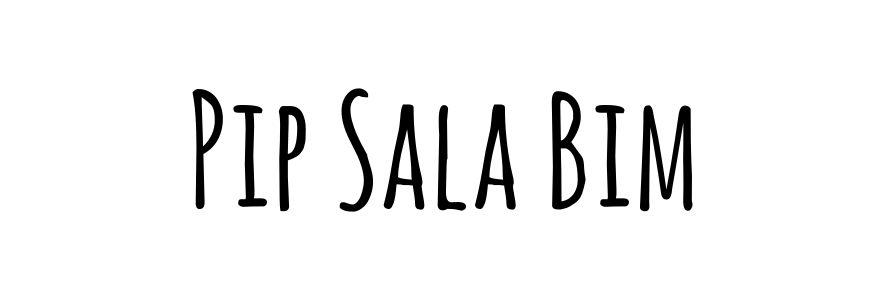
\includegraphics[width=0.200\linewidth]{../../../docs/user/rst/images/title.png}

Image with 100\% width:

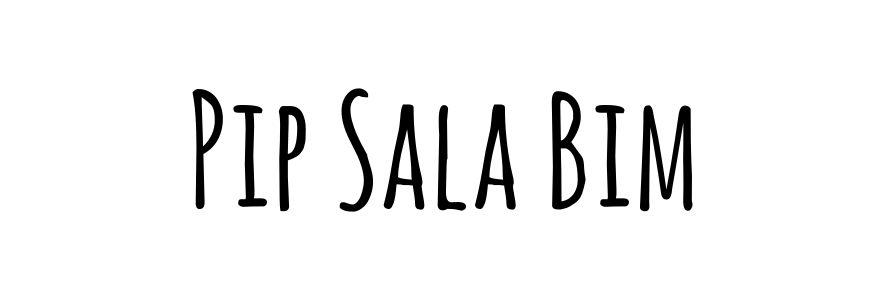
\includegraphics[width=1.000\linewidth]{../../../docs/user/rst/images/title.png}


\section{Rowspanning tables%
  \label{rowspanning-tables}%
}

Several rowspanning cells in a table.

Problem:

In LaTeX, \textquotedbl{}overwritten\textquotedbl{} cells need to be defined as empty cells.

Docutils (similarily to HTML) uses is the \textquotedbl{}Exchange Table Model\textquotedbl{} (also known
as CALS tables, see docs/ref/soextblx.dtd) which defines only the remaining
cells in a row \textquotedbl{}affected\textquotedbl{} by multirow cells.

Therefore, visit\_entry() is only called for the remaining cells and the
LaTeX writer needs bookkeeping to write out the required number of extra
'\&'s.

\setlength{\DUtablewidth}{\linewidth}
\begin{longtable*}[c]{|p{0.075\DUtablewidth}|p{0.133\DUtablewidth}|p{0.133\DUtablewidth}|p{0.086\DUtablewidth}|}
\hline

11
 & 
12
 & 
13
 & 
14
 \\
\hline

21
 & \multirow{2}{0.13\DUtablewidth}{%
2/3 2
} & \multirow{3}{0.13\DUtablewidth}{%
2…4 3
} & 
24
 \\
\cline{1-1}
\cline{4-4}

31
 &  &  & 
34
 \\
\cline{1-1}
\cline{2-2}
\cline{4-4}

41
 & 
42
 &  & 
14
 \\
\hline
\end{longtable*}

\setlength{\DUtablewidth}{\linewidth}
\begin{longtable*}[c]{|p{0.098\DUtablewidth}|p{0.098\DUtablewidth}|p{0.063\DUtablewidth}|}
\hline

11
 & 
12
 & 
13
 \\
\hline
\multirow{2}{0.10\DUtablewidth}{%
2/3 1
} & \multirow{2}{0.10\DUtablewidth}{%
2/3 2
} & 
23
 \\
\cline{3-3}
 &  & 
33
 \\
\hline
\end{longtable*}

\setlength{\DUtablewidth}{\linewidth}
\begin{longtable*}[c]{|p{0.098\DUtablewidth}|p{0.063\DUtablewidth}|}
\hline

11
 & 
12
 \\
\hline
\multirow{2}{0.10\DUtablewidth}{%
2/3 1
} & 
22
 \\
\cline{2-2}
 & 
32
 \\
\hline
\end{longtable*}

\setlength{\DUtablewidth}{\linewidth}
\begin{longtable*}[c]{|p{0.063\DUtablewidth}|p{0.110\DUtablewidth}|p{0.063\DUtablewidth}|}
\hline

11
 & 
12
 & 
13
 \\
\hline

21
 & \multirow{2}{0.11\DUtablewidth}{%
2/3 2
} & 
23
 \\
\cline{1-1}
\cline{3-3}

31
 &  & 
33
 \\
\hline
\end{longtable*}

\setlength{\DUtablewidth}{\linewidth}
\begin{longtable*}[c]{|p{0.063\DUtablewidth}|p{0.110\DUtablewidth}|}
\hline

11
 & 
12
 \\
\hline

21
 & \multirow{2}{0.11\DUtablewidth}{%
2/3 1
} \\
\cline{1-1}

31
 &  \\
\hline
\end{longtable*}

\setlength{\DUtablewidth}{\linewidth}
\begin{longtable*}[c]{|p{0.063\DUtablewidth}|p{0.110\DUtablewidth}|}
\hline

11
 & \multirow{2}{0.11\DUtablewidth}{%
1/2 1
} \\
\cline{1-1}

21
 &  \\
\hline

31
 & 
32
 \\
\hline
\end{longtable*}

\setlength{\DUtablewidth}{\linewidth}
\begin{longtable*}[c]{|p{0.063\DUtablewidth}|p{0.156\DUtablewidth}|p{0.110\DUtablewidth}|}
\hline

11
 & \multirow{2}{0.16\DUtablewidth}{%
1/2 2
} & \multirow{2}{0.11\DUtablewidth}{%
1/2 3
} \\
\cline{1-1}

21
 &  &  \\
\hline
\end{longtable*}

\setlength{\DUtablewidth}{\linewidth}
\begin{longtable*}[c]{|p{0.098\DUtablewidth}|p{0.063\DUtablewidth}|p{0.110\DUtablewidth}|}
\hline
\multirow{2}{0.10\DUtablewidth}{%
1/2 3
} & 
12
 & \multirow{2}{0.11\DUtablewidth}{%
1/2 3
} \\
\cline{2-2}
 & 
22
 &  \\
\hline
\end{longtable*}

\setlength{\DUtablewidth}{\linewidth}
\begin{longtable*}[c]{|p{0.098\DUtablewidth}|p{0.063\DUtablewidth}|}
\hline
\multirow{2}{0.10\DUtablewidth}{%
1/2 3
} & 
12
 \\
\cline{2-2}
 & 
22
 \\
\hline

31
 & 
32
 \\
\hline
\end{longtable*}

\end{document}
